\documentclass[11pt]{article}
\usepackage[margin=0.9in]{geometry}
\usepackage{fontspec}
\setmainfont{Helvetica Neue}
\newfontfamily\dev{Kohinoor Devanagari}[Script=Devanagari]
\usepackage{graphicx,booktabs,enumitem,float,array,caption}
\usepackage{xcolor}
\usepackage[colorlinks=true,urlcolor=blue!60!black,linkcolor=black]{hyperref}
\setlist{nosep,leftmargin=1.3em}
\setlength{\parindent}{0pt}\setlength{\parskip}{5pt}
\title{Audio Clip Boundaries and Transcription Methods\\for the 100 Hindi--English Listening Examples}
\author{cs-tts-steering project}
\date{November 8, 2026}
\begin{document}
\maketitle

\section*{Headline Findings}
\begin{itemize}
\item \textbf{Clip boundaries are a fundamental problem for the original romanized Hindi transcripts (O).} Most (71/100) clips match direct transcription by Whisper-Large V3. The rest (29/100) are flagged with transcription problems; 16 have clip boundary errors, where the audio is cut at the wrong place (part of the line missing, or another speaker included). The rest are word errors in the transcript (7), audio that says something else (2), garbled transcripts (2) and unclear cases (2). Manual reviews of flagged clips are in Appendix A.1.
\item \textbf{The current Devanagari transcripts (A) are the weakest version.} They were made by a simple rule-based converter (\texttt{hinlang}) from the romanized transcripts. About 40\% of Hindi words are misspelled, mostly vowel marks. This is consistent with lab members' manual listening feedback that several vowel sounds are incomplete / missing in the transcript.
\item \textbf{The LLM conversion (B) is the most promising version.} Of the four Devanagari versions converted from the same romanized text, it is the closest to what Whisper hears in the audio, on all clips and on the clean ones. It keeps English in Latin and changes nothing but the script.
\item \textbf{IndicXlit (C) does not perform as well as LLM conversion (B).} It spells long words well but gets short, common words wrong (e.g.\ \emph{ke}, \emph{to}, \emph{mai}), because it converts each word without context.
\item \textbf{Direct transcription (D) is useful as a check, but not necessarily as a replacement.} It catches content errors in O, but it also picks up other speakers at clip edges and still writes some English in Devanagari.
\end{itemize}

\section*{Five versions of MaSaC Transcripts}
\begin{tabular}{@{}l p{0.78\textwidth}@{}}
\toprule
\textbf{O} & Original romanized Hindi/English transcript. \\
\textbf{A} & Current Devanagari/English, converted from O by \texttt{hinlang} (rule-based). Used in all experiments so far. \\
\textbf{B} & LLM conversion of O (Claude Opus 5.5). Script change only: no words added, removed or corrected. \\
\textbf{C} & IndicXlit conversion of O (AI4Bharat, official package), one word at a time. \\
\textbf{D} & Direct transcription of the audio: \href{https://huggingface.co/openai/whisper-large-v3}{Whisper-large-v3}, Hindi, with a mixed-script prompt so English stays in Latin. \\
\bottomrule
\end{tabular}

B, C, D are new. B and C use the same decision about which words are English, so they differ only in how Hindi words are spelled. Prompt for D available in Appendix A.3.

\section*{First: many clips are not cleanly cut}
Before comparing transcript versions, we checked whether the original romanized transcript (O) matches its audio clip at all. We ran Whisper-large-v3 on each natural clip four ways (greedy Hindi, beam-5 Hindi, beam-5 auto-language, beam-5 English, all without a prompt), took the decode closest to the transcript, and hand-reviewed the 32 clips where even the closest decode differed by more than 0.3 (see the metric definition in the next section). Each was labelled by reading the transcript against the Whisper output; no one has listened yet.

\begin{figure}[H]\centering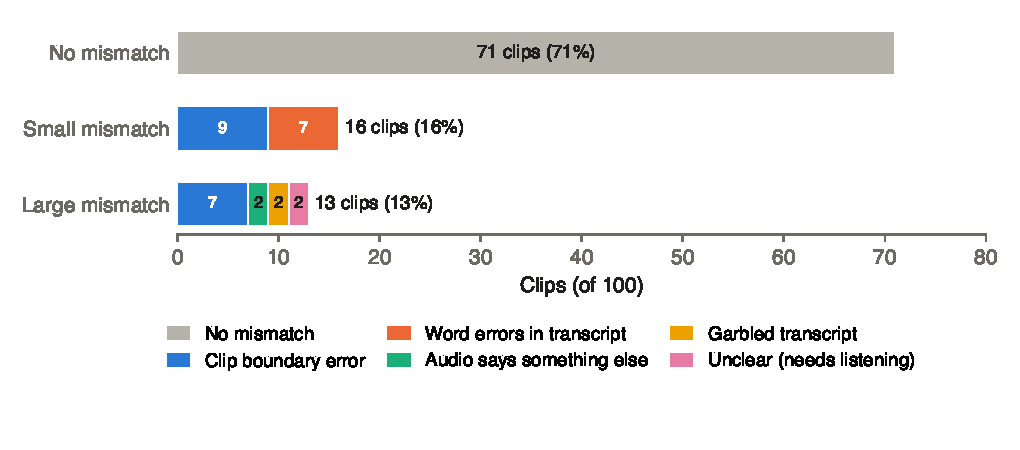
\includegraphics[width=0.82\textwidth]{fig4_match.pdf}
\caption*{\small\textbf{Figure 1.} 71 of 100 clips match their transcript with no problem. The other 29 are split by size of mismatch and coloured by possible reason. Most problems are clip boundary errors: part of the line is cut off, or another speaker's words are included at the start or end. This is a problem with the audio segmentation, not the transcript, and no spelling fix can repair it.}\end{figure}

\subsection*{Flagged clips (29 of 100)}
Flagged clips are split by how much of the line is affected, and each has a possible reason:
\begin{itemize}
\item \textbf{Large}: most of the line in O does not match what Whisper hears (normalised CER typically above 0.55). O cannot be used as is; re-transcribe, re-cut the clip, or drop it.
\item \textbf{Small}: the mismatch is limited to a few words, at the edge of the clip or within the line (CER about 0.3--0.5). O is usable after a small fix.
\end{itemize}
The sizes are judgment calls made by reading the transcript against Whisper's output; so are the reasons. Please confirm or correct both after listening.

The full lists, with a column for manual review, are in Appendix A.1.

\section*{How the versions compare}
We use D as a stand-in for ``what is actually said'' and measure how far each version is from it. The measure is a \textbf{normalised character error rate (CER)}, computed per clip:
\begin{enumerate}
\item \textbf{Same script.} Both texts are converted to Latin letters with \texttt{uroman} (Devanagari $\rightarrow$ Latin; Latin text is unchanged), lowercased, and punctuation is removed.
\item \textbf{Ignore spelling-only differences.} Within each word: \emph{ee}$\rightarrow$\emph{i}, \emph{oo}$\rightarrow$\emph{u}, \emph{ai}$\rightarrow$\emph{e}, \emph{au}$\rightarrow$\emph{o}, \emph{y}$\rightarrow$\emph{i}; the letter \emph{h} is dropped (so aspiration doesn't count); doubled letters are collapsed; \emph{f}$\rightarrow$\emph{ph}, \emph{q}$\rightarrow$\emph{k}, \emph{z}$\rightarrow$\emph{j}, \emph{w}$\rightarrow$\emph{v}, \emph{x}$\rightarrow$\emph{ks}, \emph{c}$\rightarrow$\emph{k}.
\item \textbf{Count edits.} Spaces are removed, and CER = (insertions + deletions + substitutions needed to turn the version into D) $\div$ (number of characters in the version). 0 means identical after normalisation; 0.2 means about one character in five differs.
\end{enumerate}
The bars show the median CER over clips. Because step 2 forgives many spelling differences (e.g.\ vowel length), this measure mainly tests whether the \emph{words} match, and it understates A's vowel errors (Figure 4 counts those directly). D is not ground truth, so these are relative comparisons.

\begin{figure}[H]\centering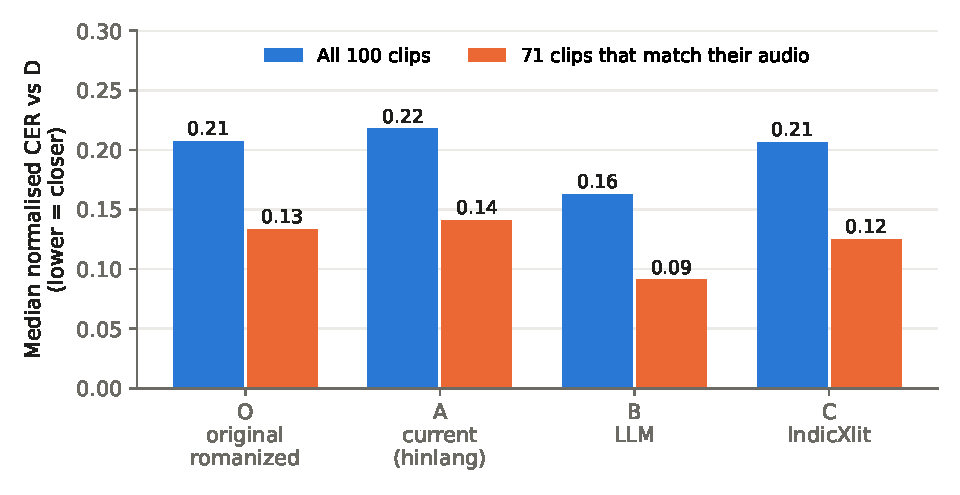
\includegraphics[width=0.72\textwidth]{fig1_closeness.pdf}
\caption*{\small\textbf{Figure 2.} Median normalised CER against the direct transcription (D). B is closest. On the 71 clips that match their audio, B's difference is about a third lower than A's.}\end{figure}

\begin{figure}[H]\centering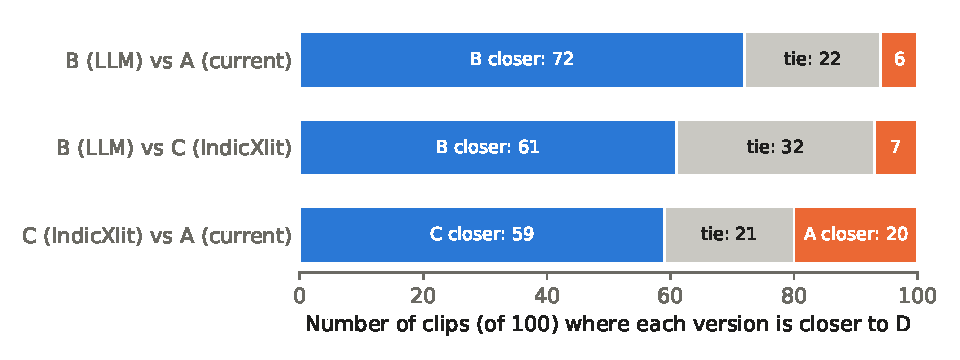
\includegraphics[width=0.72\textwidth]{fig2_headtohead.pdf}
\caption*{\small\textbf{Figure 3.} Clip-by-clip: which version is closer to D. B beats A on 72 clips and loses on 6; B beats C on 61 and loses on 7. Ties are clips where both versions are equally close.}\end{figure}

\begin{figure}[H]\centering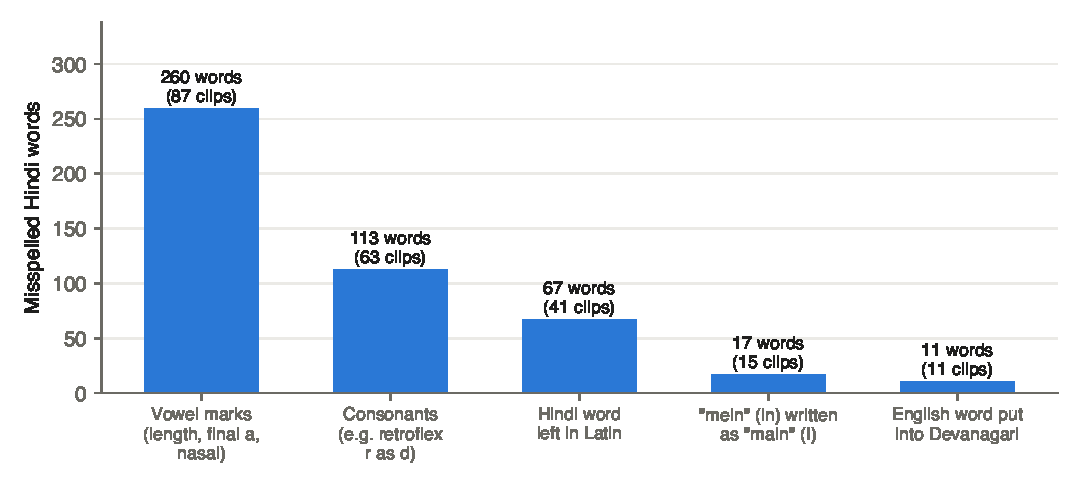
\includegraphics[width=0.8\textwidth]{fig3_errors.pdf}
\caption*{\small\textbf{Figure 4.} What goes wrong in the current version (A), compared with a careful re-conversion. Vowel marks are the biggest problem, which fits the listener's comment that vowels sound missing in TTS output.}\end{figure}


\section*{What we noticed}
\begin{itemize}
\item \textbf{The old converter has a few systematic bugs.} ``mein'' (in) always becomes ``main'' (I); retroflex sounds are written as plain d; final vowels are dropped (\emph{kaha} $\rightarrow$ \emph{kah}); and words are put in the wrong script whenever the automatic language tagger is wrong.
\item \textbf{IndicXlit's errors are predictable.} Almost all are short function words. A small exception list would fix most of them and make C a reproducible alternative to B.
\item \textbf{B is not perfectly reproducible.} Re-running the LLM won't give byte-identical output, so the version we use should be saved and proofread once.
\item \textbf{The mixed-script prompt made D comparable.} Without it Whisper wrote 16\% of English words in Latin; with it, 64\%.
\item \textbf{Earlier high Whisper error rates were partly Whisper's fault.} Some clips scored very badly because Whisper got stuck repeating a word, not because the transcript was wrong.
\end{itemize}

\section*{Recommendation}
\begin{enumerate}
\item We are still awaiting manual feedback from Kavya (sent Sun, Nov. 8) on the 5 transcript samples. 
\item Tentatively leading towards adopting \textbf{B (LLM)} as the Devanagari input, after a one-time proofread by a Hindi speaker on select clips (about 1--2 hours for 100 clips).
\item Use \textbf{D} only to flag clips where O may be wrong, then check those clips by ear or rule them out from the train / test set.
\item Listen to the 29 flagged clips and fill in the Manual review column (Appendix A.1). Re-cut the clip boundary errors, fix the word errors, and re-transcribe or drop the rest.
\end{enumerate}

\enlargethispage{3\baselineskip}
\section*{Caveats}
\begin{itemize}
\item All audio-match judgments come from Whisper, which is weak on Hinglish. No one has listened yet.
\item Comparing against Whisper favours standard spellings, which helps B and C regardless of what was said.
\item D can include speech from neighbouring speakers at the clip edges.
\end{itemize}
\clearpage
\section*{Appendix}
\subsection*{A.1\quad Manual review of mismatched clips}
Listen to each clip and confirm or correct the size and possible reason in the Manual review column. Definitions of Large and Small are in the section ``First: many clips are not cleanly cut''.

\subsubsection*{Large mismatch (13 clips)}
\begin{center}\begin{tabular}{@{}p{0.2\textwidth} p{0.1\textwidth} p{0.3\textwidth} p{0.3\textwidth}@{}}
\toprule
\textbf{Folder} & \textbf{Split} & \textbf{Possible reason} & \textbf{Manual review}\\
\midrule
\texttt{03\_train\_1440\_3} & dev & Clip boundary error & \rule{0.28\textwidth}{0.4pt}\\
\texttt{06\_train\_685\_4} & train & Clip boundary error & \rule{0.28\textwidth}{0.4pt}\\
\texttt{12\_val\_205\_5} & train & Clip boundary error & \rule{0.28\textwidth}{0.4pt}\\
\texttt{14\_train\_1753\_4} & test & Clip boundary error & \rule{0.28\textwidth}{0.4pt}\\
\texttt{56\_train\_1421\_3} & train & Clip boundary error & \rule{0.28\textwidth}{0.4pt}\\
\texttt{86\_train\_497\_4} & train & Clip boundary error & \rule{0.28\textwidth}{0.4pt}\\
\texttt{87\_train\_612\_3} & train & Clip boundary error & \rule{0.28\textwidth}{0.4pt}\\
\texttt{83\_train\_755\_0} & dev & Audio says something else & \rule{0.28\textwidth}{0.4pt}\\
\texttt{85\_train\_663\_3} & train & Audio says something else & \rule{0.28\textwidth}{0.4pt}\\
\texttt{58\_train\_90\_1} & train & Garbled transcript & \rule{0.28\textwidth}{0.4pt}\\
\texttt{97\_test\_82\_2} & excluded & Garbled transcript & \rule{0.28\textwidth}{0.4pt}\\
\texttt{42\_train\_986\_7} & train & Unclear (needs listening) & \rule{0.28\textwidth}{0.4pt}\\
\texttt{66\_val\_124\_0} & train & Unclear (needs listening) & \rule{0.28\textwidth}{0.4pt}\\
\bottomrule\end{tabular}\end{center}

\subsubsection*{Small mismatch (16 clips)}
\begin{center}\begin{tabular}{@{}p{0.2\textwidth} p{0.1\textwidth} p{0.3\textwidth} p{0.3\textwidth}@{}}
\toprule
\textbf{Folder} & \textbf{Split} & \textbf{Possible reason} & \textbf{Manual review}\\
\midrule
\texttt{16\_train\_1060\_0} & train & Clip boundary error & \rule{0.28\textwidth}{0.4pt}\\
\texttt{25\_train\_1251\_3} & train & Clip boundary error & \rule{0.28\textwidth}{0.4pt}\\
\texttt{30\_train\_357\_0} & train & Clip boundary error & \rule{0.28\textwidth}{0.4pt}\\
\texttt{40\_train\_1693\_0} & test & Clip boundary error & \rule{0.28\textwidth}{0.4pt}\\
\texttt{53\_train\_1439\_1} & dev & Clip boundary error & \rule{0.28\textwidth}{0.4pt}\\
\texttt{69\_train\_1390\_0} & train & Clip boundary error & \rule{0.28\textwidth}{0.4pt}\\
\texttt{71\_train\_1179\_6} & train & Clip boundary error & \rule{0.28\textwidth}{0.4pt}\\
\texttt{82\_train\_477\_2} & train & Clip boundary error & \rule{0.28\textwidth}{0.4pt}\\
\texttt{95\_train\_757\_1} & train & Clip boundary error & \rule{0.28\textwidth}{0.4pt}\\
\texttt{31\_test\_39\_1} & train & Word errors in transcript & \rule{0.28\textwidth}{0.4pt}\\
\texttt{46\_val\_192\_2} & train & Word errors in transcript & \rule{0.28\textwidth}{0.4pt}\\
\texttt{49\_train\_1221\_7} & train & Word errors in transcript & \rule{0.28\textwidth}{0.4pt}\\
\texttt{50\_train\_1574\_0} & test & Word errors in transcript & \rule{0.28\textwidth}{0.4pt}\\
\texttt{59\_train\_1000\_6} & train & Word errors in transcript & \rule{0.28\textwidth}{0.4pt}\\
\texttt{63\_train\_1222\_2} & dev & Word errors in transcript & \rule{0.28\textwidth}{0.4pt}\\
\texttt{67\_train\_1378\_23} & train & Word errors in transcript & \rule{0.28\textwidth}{0.4pt}\\
\bottomrule\end{tabular}\end{center}

Folder names refer to \texttt{Listening\_Examples\_100\_PT/} on kedi (the folder name continues with the first words of the transcript). \texttt{test\_82\_2} is already excluded from the experiments.


\subsection*{A.2\quad The five samples sent for labeling}
Natural clips were sent out to Kavya, Debasmita, and Alehsan on Sunday Nov 8th.

\subsubsection*{1.\ \texttt{92\_train\_1355\_2} (dev) --- many long vowels}
\begin{tabular}{@{}l p{0.9\textwidth}@{}}
\textbf{O} & {\dev Maya, mai to kahata hu agar chain se sona hai na, to use utha ke baahar fek dena chaahiye!}\\
\textbf{A} & {\dev मय, मैं तो कहत हूँ अगर चिन से सोन है ना, तो उसे उथ के बाहर फेक देना चहिये!}\\
\textbf{B} & {\dev माया, मैं तो कहता हूँ अगर चैन से सोना है ना, तो उसे उठा के बाहर फेंक देना चाहिए!}\\
\textbf{C} & {\dev माया, माई टो कहता हू अगर चैन से सोना है ना, टो उसे उठा केई बाहर फेक देना चाहिये!}\\
\textbf{D} & {\dev माया, मैं तो कहता हूँ, अगर चैन से सोना है ना, तो उसे उठा के बाहर तेक देना चाहिए. नहीं, नहीं.}\\
\end{tabular}

\subsubsection*{2.\ \texttt{29\_train\_101\_5} (dev) --- retroflex sounds and ``mein''}
\begin{tabular}{@{}l p{0.9\textwidth}@{}}
\textbf{O} & {\dev Jis ke mukaabale meri momma, baajre ke khet mein khadi scarecrow jaisi lagti hai?}\\
\textbf{A} & {\dev जिस के मुकाबले मेरी momma, बाज्रे के खेत मैं ख्दि scarecrow जैसि लग्ति है?}\\
\textbf{B} & {\dev जिस के मुक़ाबले मेरी momma, बाजरे के खेत में खड़ी scarecrow जैसी लगती है?}\\
\textbf{C} & {\dev जिस केई मुकाबले मेरी momma, बाजरे केई खेत में खादी scarecrow जैसी लगती है?}\\
\textbf{D} & {\dev जिसके मुकाबले मेरी मॉमा बाजरे के खेत में खड़ी scarecrow जैसी लगती है.}\\
\end{tabular}

\subsubsection*{3.\ \texttt{39\_train\_588\_5} (test) --- heavy code-switching}
\begin{tabular}{@{}l p{0.9\textwidth}@{}}
\textbf{O} & {\dev Don't be ridiculous Sahil, ek party mein jaane ke liye mai aisi childish games nahi khelungi! excuse me!}\\
\textbf{A} & {\dev Don't be ridiculous सहिल, एक party मैं जाने के लिये मैं ऐसि childish games नहीं खेलुंगि! excuse me!}\\
\textbf{B} & {\dev Don't be ridiculous साहिल, एक party में जाने के लिए मैं ऐसी childish games नहीं खेलूँगी! excuse me!}\\
\textbf{C} & {\dev Don't be ridiculous साहिल, एक party में जाने केई लिये माई आइसी childish games नही खेलूंगी! excuse me!}\\
\textbf{D} & {\dev Don't be ridiculous, साहिल. एक party में जाने के लिए मैं ऐसी childish games नहीं खेलूंगी, excuse me.}\\
\end{tabular}

\subsubsection*{4.\ \texttt{80\_val\_18\_3} (dev) --- the versions disagree most}
\begin{tabular}{@{}l p{0.9\textwidth}@{}}
\textbf{O} & {\dev Thodi jidd karungi to candles free me de denge vo log.}\\
\textbf{A} & {\dev थोड़ी जिद्द करुंगि to candles free me de देंगे वो log.}\\
\textbf{B} & {\dev थोड़ी ज़िद करूँगी तो candles free में दे देंगे वो लोग.}\\
\textbf{C} & {\dev थोड़ी जिद्द करूंगी टो candles free मे डीई डेंगे वो लॉग.}\\
\textbf{D} & {\dev थोड़ी जित करूँगी, तो candles फ्री में दे देंगे वो लोग.}\\
\end{tabular}

\subsubsection*{5.\ \texttt{50\_train\_1574\_0} (test) --- possible wrong word in the original}
\begin{tabular}{@{}l p{0.9\textwidth}@{}}
\textbf{O} & {\dev Mujhe sach bataao, vo akhir doctor hai?}\\
\textbf{A} & {\dev मुझे सच बताओ, वो अखिर doctor है?}\\
\textbf{B} & {\dev मुझे सच बताओ, वो आख़िर doctor है?}\\
\textbf{C} & {\dev मुझे सच बताओ, वो अखीर doctor है?}\\
\textbf{D} & {\dev सच बता, वो वाकर ही doctor है.}\\
\end{tabular}

\subsection*{A.3\quad Whisper-large-v3 mixed-script prompt (version D)}
Full decoder prompt given to Whisper-large-v3 for every clip (124 tokens; the audio goes to the encoder separately; beam 5), verbatim:
\begin{quote}\raggedright\hyphenpenalty=10000\exhyphenpenalty=10000
\texttt{<|startofprev|>}{\dev\ हाँ यार, आज office में बहुत काम था, लेकिन meeting cancel हो गई. Actually मुझे लगा कि boss नाराज़ होंगे, पर सब ठीक-ठाक रहा. चलो, weekend पे movie देखते हैं, okay?}\allowbreak\texttt{<|startoftranscript|>}\allowbreak\texttt{<|hi|>}\allowbreak\texttt{<|transcribe|>}\allowbreak\texttt{<|notimestamps|>}
\end{quote}
Whisper writes its transcript after the last token.

\end{document}